\section{Blazor Maui}
\label{sec:blazormaui}
Mit dem Release von .Net 6 wurde Blazor mit Maui kombiniert. Die Abkürzung \emph{Maui} steht dabei
für \emph{Multi-platform Application UI}. Mit
Blazor Maui sollen zukünftig native Desktop-  oder Mobile Applikationen mit Blazor erstellt werden
können.
\newline
\newline
Die Architektur von Blazor Maui sieht vor, dass der Blazor Code durch Maui in nativen Code
umgewandelt wird. Dieser kann dadurch auf der jeweiligen Platform ausgeführt zu werden. Was im
folgenden Bild zu erkennen ist:
\newpage
\begin{figure}[h]
    \centering
    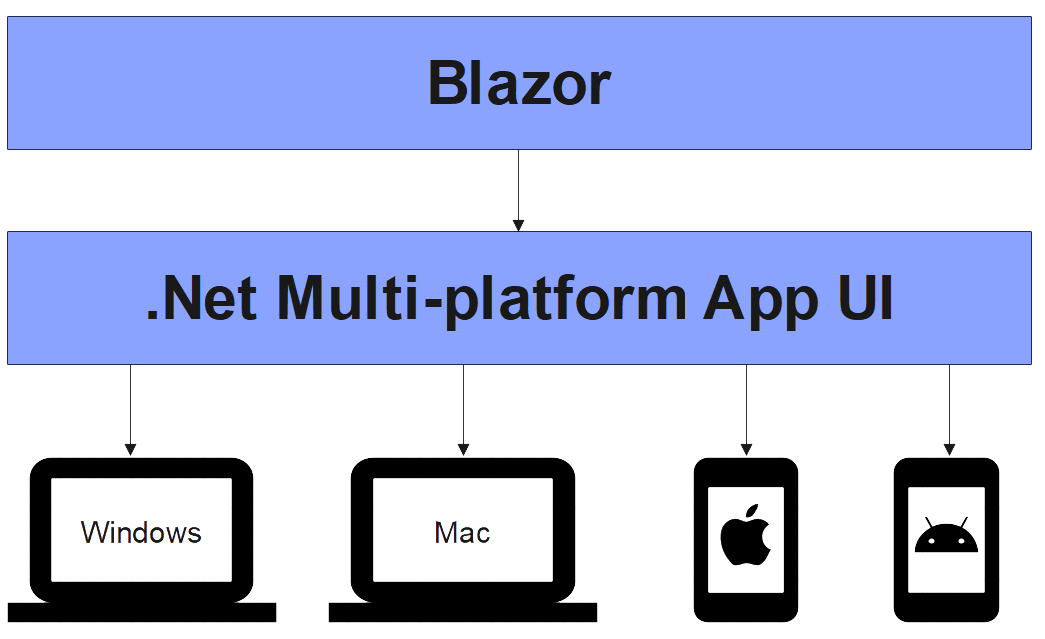
\includegraphics[width=\textwidth, center]{Blazor/BlazorMaui}
    \caption[Blazor Maui Architektur]{Blazor Maui Architektur}
    \label{img:BlazorMaui}
\end{figure}

Wie zu sehen ist, werden Windows, Mac, iOS und Android mithilfe von Maui untersützt. Linux
hingegen bleibt zu dem Zeitpunkt dieser Arbeit noch außen vor.
\newline
\newline
Aufgrund dessen, das Linux zum derweiligen Zeitpunkt noch nicht unterstützt wird, und Non-Deeply
Embedded System meist auf Linux basieren, wird Blazor Maui nicht weitergehend in dieser Arbeit
behandelt.